\documentclass[a4paper,12pt]{article}
\usepackage[pdftex]{graphicx}
\usepackage[margin=2cm]{geometry}
\usepackage{amsmath}
%
%--------------------   start of the 'preamble'
\newtheorem{defn}{Definition}
%---------------------   end of the 'preamble'
%
\begin{document}
%-----------------------------------------------------------
\title{Evaluation Criteria for NET-VISA and SIG-VISA Prototypes for
  Detection, Identification, and Association of Seismic Data}
\author{Nimar S. Arora 
\\University of California, Berkeley \\ nimar@cs.berkeley.edu
\and Stuart Russell 
\\University of California, Berkeley  \\ russell@cs.berkeley.edu
 \and Erik Sudderth \\ Brown University \\ sudderth@cs.brown.edu }
\maketitle

\abstract{We present evaluation criteria for judging the quality of a computer-generated seismic event
  bulletin when compared with a ground-truth bulletin. The criteria
  are based on computing a bipartite matching between the events in the
  two bulletins and reporting the precision, recall, and average error in distance, time, and magnitude.
  We justify the relevance of the criteria for treaty
  monitoring purposes and demonstrate on a few examples. 
  Although this document is mainly concerned with the evaluation of a single
  NET-VISA or SIG-VISA bulletin when compared against the LEB bulletin
  for the whole earth, the criteria are easily extended to the case of
  a local or regional ground-truth bulletin and also
  to the task of evaluating a distribution over bulletins.}

\section{Introduction}

The Preparatory Commission for the Comprehensive Nuclear-Test-Ban Treaty
Organization (CTBTO) operates a globally distributed network of
seismic, hydroacoustic, and infrasound stations. These stations, and
the associated communications system, are together known
as the International Monitoring System (IMS). Time series data from these
stations are received at the CTBTO's International Data Center (IDC),
where they are processed automatically and interactively using the IDC
application software. The automatic phase of the processing produces the
seismic event bulletins SEL1, SEL2, and SEL3. These bulletins are
reviewed by analysts who produce a bulletin known as the LEB. The LEB is
subsequently filtered to produce the Reviewed Event Bulletin (REB).

Vertically Integrated Seismological Analysis (VISA) is an algorithmic
approach to seismic processing based on a probabilistic generative
model of event creation, transmission of seismic waves, and the
generation of seismic waveforms at the stations. Its first
instantiation in a computer program, NET-VISA, covers just the network
processing phase; that is, its generative model predicts just the {\em
  detections} caused by seismic (and noise) events, rather than the
full seismic waveforms, and it takes as input the detections as
produced by the IDC DFX software. The next instantiation of VISA,
known as SIG-VISA, will incorporate a generative model of raw signal
characteristics, bypassing the detection step. The model parameters of
VISA are estimated from historical data and inference uses various
approaches including Markov Chain Monte Carlo and stochastic search.

The purpose of this document is to describe the attributes of a seismic
bulletin and an evaluation criterion based on bipartite matching. The
same criteria can be used for evaluating other seismic bulletins as
well, for instance SEL3.

\section{Seismic Bulletin Evaluation: Background and Motivation}
\label{sec-eval}

For our current purposes, we define a {\em seismic event bulletin} as a set of events in a specified
space--time region with the following attributes for each event:
longitude, latitude, depth, time, and magnitude (body-wave magnitude,
$m_b$). A bulletin may consist of {\em predicted} events (as generated
by a computer program, for example) or {\em ground-truth} events (as
determined by human experts, for example, perhaps with the aid of
dense local networks and direct reports for man-made events).
We are interested in the numbers of real and spurious events
in the bulletin, and in how many real events are omitted, when the
bulletin is compared to ground truth. For the real events, we are also
interested in the accuracy of the event parameters.

In general, the design of evaluation criteria for seismic bulletins
(and the software that generates them) depends on their intended
context of use. For CTBTO, the output of the automated processing
stage is intended to provide input for an analyst review stage, which
makes it difficult to justify any particular set of criteria on
quantitative analytic grounds. Questions such as ``How useful is the
automated bulletin in helping the analysts find the real events?'' and
``How much bias does it introduce in the process?'' do not have
analytical answers; these can only be answered empirically based on
experience in realistic use.

The operation of the VISA algorithms is unaffected by the thresholds
used for evaluation, so it is straightforward to report VISA's
performance under a wide range of criteria if necessary.

\subsection{Matching single events}

The concepts of ``real'' and ``spurious'' predicted events presume
that a hard distinction between the two is possible, given ground
truth.  Because predicted events hardly ever match ground truth {\em
  exactly}, we adopt a threshold criterion based on proximity in space
and time to an event in the ground-truth bulletin. For example, we
might say that a predicted event is a {\em possible match} for a real
event if the locations lie within a distance $\delta$ and the times
are within $\tau$. In our work so far, we have used a $\delta = 5$
degrees (great-circle distance, ignoring depth) and $\tau = 50$
seconds, although of course other thresholds are possible.
The distance--time ratio of 10 seconds per degree, chosen after
discussions with analysts, reflects typical propagation velocities.

We have omitted depth disparity from this calculation because 1) depth
estimates in both SEL3 and LEB are unreliable for smaller events, and 2) the
primary purpose of the IMS is to detect possible nuclear explosions,
which have depth zero, so the accuracy of depth estimates for deep
events is less important, while accurate waveform association and
hence accurate time are required for event type classification and
magnitude estimation and accurate latitude and
longitude are required for OSI.

Given the well-known problem of depth/time aliasing for events with
only teleseismic detections, it might be reasonable to include depth
in the matching threshold definition but to make an appropriate
allowance for depth/time errors.


\subsection{Matching multiple events}

A {\em possible} match is not the same as an {\em actual} match
because a bulletin could have multiple predicted events that
possibly match a single ground-truth event. Moreover, a predicted event might be in the vicinity of multiple
ground-truth events and cannot be construed as a successful detection
of more than one of them. A natural solution is to construct a {\em
  matching} between between the two sets of predicted and ground-truth
events, such that each predicted event matches at most one
ground-truth event within its $(\delta,\tau)$ space-time region and vice versa. (Formal definitions are given
below.) Then we say that an event is real (in a given matching) if it
is matched to a ground-truth event.

Figure~\ref{fig-2-bulletins} illustrates these concepts in a
simplified context where events are located in a 2D space--time plane.
In the figure, the predicted event $1$ is clearly not real
and the ground truth event $C$ is not recovered (it has no possible
matches). However, the picture is
a bit muddled for the other events. We could claim that event $2$
matches event $B$ in which case events $3$ and $4$ would not be real and
event $A$ would not be recovered. A more sensible choice for
evaluation purposes is to maximize the number of matched ground-truth
events---a {\em max-cardinality} matching. There are two such
matchings here: we could match $2$ to $A$ and $3$ to $B$, or $2$ to
$A$ and $4$ to $B$. Of these two max-cardinality matchings,
we may prefer the latter because $4$ is ``closer'' to $B$ in
space--time than $3$ is, given the chosen distance metric.
In general, then, we evaluate a bulletin by the quality of
its {\em min-weight max-cardinality matching} to ground truth, where
the weight is computed from the space--time distances of all the
matched pairs in the matching.

\begin{figure}
\begin{center}
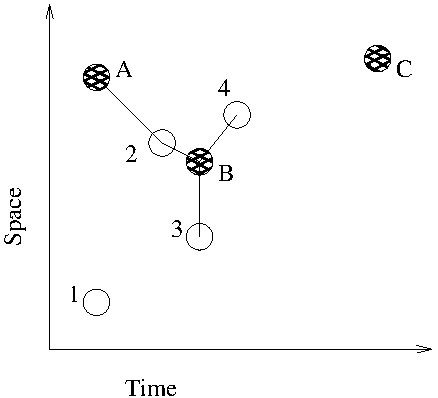
\includegraphics{visa_eval_fig1.pdf}
\end{center}
\caption{Graphical depiction of two bulletins: predicted events
  (empty circles 1, 2, 3, 4) and ground-truth events (shaded circles
  A, B, C). Lines connect predicted and ground-truth events
  that {\em possibly match}---i.e., are close enough to each other.}
\label{fig-2-bulletins}
\end{figure}

\subsection{Ground-truth bulletins}

The choice of the ground-truth bulletin is clearly critical in the
evaluation. Since the LEB is produced by expert human analysts,
it is a reasonable default choice. It is worth noting, however, that
using LEB as ground truth when comparing the accuracy of SEL3 and VISA
bulletins introduced a bias in favor of SEL3 because LEB 
is constructed with the SEL3 as input and hence tends to
include events from SEL3, in particular, low magnitude events, and to
exclude events that are not in SEL3 since these require much more work
on the part of the analysts to find and confirm. One reasonable
alternative might be to construct a new LEB$^*$ from the
combined SEL3 and VISA bulletins (with duplicate events removed).
Obviously this would incur additional costs in analyst time.

Some of our experiments with VISA have shown that it can find events
that do not appear in LEB but are confirmed in other bulletins based
on dense regional networks, such as NEIC. Such bulletins could be used
to conduct a more ``objective'' comparison of VISA and SEL3, although
both programs would typically exhibit low recall because the IMS is
much sparser than typical regional and local networks.


\section{Seismic Bulletin Evaluation}

\subsection{Formal Definitions}

We now provide exact definitions of the criteria we use currently for
evaluating VISA against LEB.

\begin{defn}
An undirected graph $G=(V,E)$ consists of a set of vertices $V$ and a set
of edges $E$ where an element of $E$ is a set of two vertices $\{u,v\}$,
s.t. $u,v \in V$.
\end{defn}

\begin{defn}
A bipartite graph is an undirected graph where the set of vertices $V$
can be partitioned into two subsets $V_1$, $V_2$ such that for every edge
$\{u,v\} \in E$,  $(u \in V_1 \wedge v \in V_2) \vee ( u \in V_2 \wedge v \in
V_1)$.
\end{defn}

\begin{defn}
A matching $M$ in a graph $G$ is a subset of the edges of $G$ such
that for any two edges $e_1$, $e_2$ in $M$, $e_1 \cap e_2 = \phi$. The
cardinality, $|M|$, of the matching is the number of edges in it.
\end{defn}

\begin{defn}
A weighted graph $G=(V,E,W)$ has a map $W : E \rightarrow \mathcal{R}$
that assigns a real-valued weight to each edge. By extension, the weight 
$W(M)$ of a matching,
$M$, is defined as the sum of the weights of the edges in it.
\end{defn}

\noindent The next few definitions describe a bipartite matching of seismic
bulletins.

\begin{defn}
An event $b$ is a tuple $(b^{lon}, b^{lat},
b^{depth}, b^{time}, b^{mag})$ of longitude, latitude,
depth, time, and magnitude.
A seismic bulletin $B=\{b_1, b_2,\ldots \}$ is (loosely) defined as a
set of events. The cardinality, $|B|$, of the bulletin is the number of events
in it.
\end{defn}

\noindent Strictly speaking a bulletin must also be associated with a
time interval $[t_1,t_2]$ and represents the
hypothesis that all and only those events took place in that time
interval; for most purposes, we will be comparing bulletins over the
same time interval. Similar considerations apply to bulletins defined
over specific regions.

\begin{defn}
The distance between two events $b$ and $c$, denoted $dist_{deg}(b,c)$ is the
great circle distance between the points $(b^{lon}, b^{lat})$ and
$(c^{lon}, c^{lat})$ on the surface of the earth in
degrees. $dist_{km}(b,c)$ is the same quantity measured in kilometres.
\end{defn}

\begin{defn}
A bipartite matching of two bulletins $B$ and $C$ with identical time
intervals is a matching over the
weighted bipartite graph $G=(V,E,W)$, where $V=B \cup C$, $E=\{\{b_i,
c_j\}: b_i \in B, c_j \in
C,\ dist_{deg}(b,c)<\delta,\ |b^{time}-c^{time}|<\tau \}$, and 
$W(b,c) = \frac{dist_{deg}(b,c)}{\delta} +  \frac{|b^{time} - c^{time}|}{\tau}$.
\end{defn}

The evaluation criteria for a predicted event bulletin $B$ and a ground
truth event bulletin $C$ comprise five numbers---precision,
recall, and average error in distance, time, and magnitude, which are defined as follows. Let $M$ be a
minimum-weight maximum-cardinality bipartite matching of the bulletins
$B$ and $C$, for a given choice of $\delta$ and $\tau$. Then 
\begin{align*}
\mbox{precision}(B,C) &= \frac{|M|}{|B|} \\
\mbox{recall}(B,C) &= \frac{|M|}{|C|} \\
\mbox{dist-error}(B,C) &= \frac{1}{|M|} \sum_{\{b,c\} \in M} dist_{km}(b,c) \\
\mbox{time-error}(B,C) &= \frac{1}{|M|}\sum_{\{b,c\} \in M} |b^{time} - c ^{time}| \\
\mbox{mag-error}(B,C) &= \frac{1}{|M|}\sum_{\{b,c\} \in M} |b^{mag} - c ^{mag}|.
\end{align*}
Because the goal is to detect events, it might be thought that
recall---the fraction of true events that are detected---is the most
important criterion. On the other hand, high recall can be achieved at
the expense of low precision by predicting events in every cell of a
fine space--time grid. Every detection system can achieve some form of
precision--recall tradeoff by adjusting an internal threshold for
declaring an event; thus, we will report the tradeoff achievable by
VISA using a precision--recall curve. Average error can then be
reported from a system operating at some particular point chosen along
that curve. All of these results can be reported for various choices of $\delta$ and $\tau$.

\subsection{Probabilistic bulletins}

As a natural consequence of the uncertainty in the transmission and
detections of seismic signals which is modeled by VISA, inference might
produce not just one best bulletin, but instead a posterior distribution $P(B|E)$ over
the set ${\cal B}$ of all possible bulletins, given the evidence $E$. 
In this case, the evaluation criteria given above can be applied on the bulletin
with the highest posterior probability.

\end{document}
